\documentclass[a4paper]{article}

%% Language and font encodings
\usepackage{polski}
\usepackage[polish]{babel}
\usepackage[utf8x]{inputenc}
\usepackage[T1]{fontenc}
\usepackage{pdfpages}
\usepackage{indentfirst}
\usepackage{listings}
\usepackage{isotope}

\usepackage{csvsimple}
\setlength{\tabcolsep}{2pt}

% Adjust penalties
\brokenpenalty=1000
\clubpenalty=1000
\widowpenalty=1000

% Don't break in math expressions
\relpenalty=10000
\binoppenalty=10000

%% Sets page size and margins
\usepackage[a4paper]{geometry}

%% Useful packages
\usepackage{amsmath}
\usepackage{graphicx}
\usepackage[colorlinks=true, allcolors=blue]{hyperref}
\usepackage{booktabs}
\usepackage{cancel}
\usepackage{tikz}

\usepackage{float}

\renewcommand\thesection{\arabic{section}.}
\renewcommand\thesubsection{\arabic{section}.\arabic{subsection}.}
\renewcommand\thesubsubsection{\arabic{section}.\arabic{subsection}.\arabic{subsubsection}.}

% The following commands are not supported in PSTricks at present
% We define them conditionally, so when they are implemented,
% this pgf file will use them.
\ifx\du\undefined
  \newlength{\du}
\fi
\setlength{\du}{15\unitlength}

\newcommand{\Vsp}[1]{\vtop to #1 {}}
\newcommand{\Hsp}[1]{\hbox to #1 {}}
\newcommand{\Small}{\scriptsize}

\title{Sprawozdanie nr 8}
\date{}


\begin{document}

\begin{center}
\begin{tabular}{|p{5.5cm}|l|l|c|}
    \hline
	% Row 1.1  
	    Wydział \Vsp{4mm} &
	    \multicolumn{1}{|l}{Dzień} &
	    poniedziałek $17^{15} - 19^{30}$ &
	    Nr zespołu \\
	% Row 1.2
	    \mbox{\small{Matematyki i Nauk Informatycznych}} &
	    \multicolumn{1}{|l}{Data}  &
	    &
	    \multicolumn{1}{c|}{\Large{18}} \\
    
    \hline
	% Row 2.1 
	    Nazwisko i Imię: &
	    \Small Ocena z przygotowania &
	    \Small Ocena ze sprawozdania &
	    \Small Ocena Końcowa \\
	% Rows 2.2-2.4
	    1. Jasiński Bartosz & & &\\
	    2. Sadłocha Adrian & & & \\
	    3. Wódkiewicz Andrzej & & & \\

    \hline
    % Row 3.1
	    \multicolumn{2}{|l|}{Prowadzący \Vsp{4mm}} &
	    \multicolumn{2}{|l|}{Podpis prowadzącego} \\  
    % Row 3.2
    	\multicolumn{2}{|l|}{dr hab. Jacek Gosk} &
    	\multicolumn{2}{|l|}{} \\    	
    \hline
\end{tabular}
\label{pieczatka}
\end{center}

{\let\newpage\relax\maketitle}
\setcounter{secnumdepth}{2}


\section{Opis ćwiczenia i wstęp teoretyczny}

Celem ćwiczenia było zapoznanie się z działaniem lampy elektronowej, wykazanie zależności 
natężenia prądu anodowego diody od napięcia przyłożonego na diodę oraz wyznaczenie temperatury katody
na podstawie wykonanych pomiarów.

Przed rozpoczęciem ćwiczenia, w sali laboratoryjnej przygotowany został uprzednio układ pomiarowy,
którego schemat przedstawiono na rysunku \ref{schemat}.

% \begin{figure}
% \centering
% 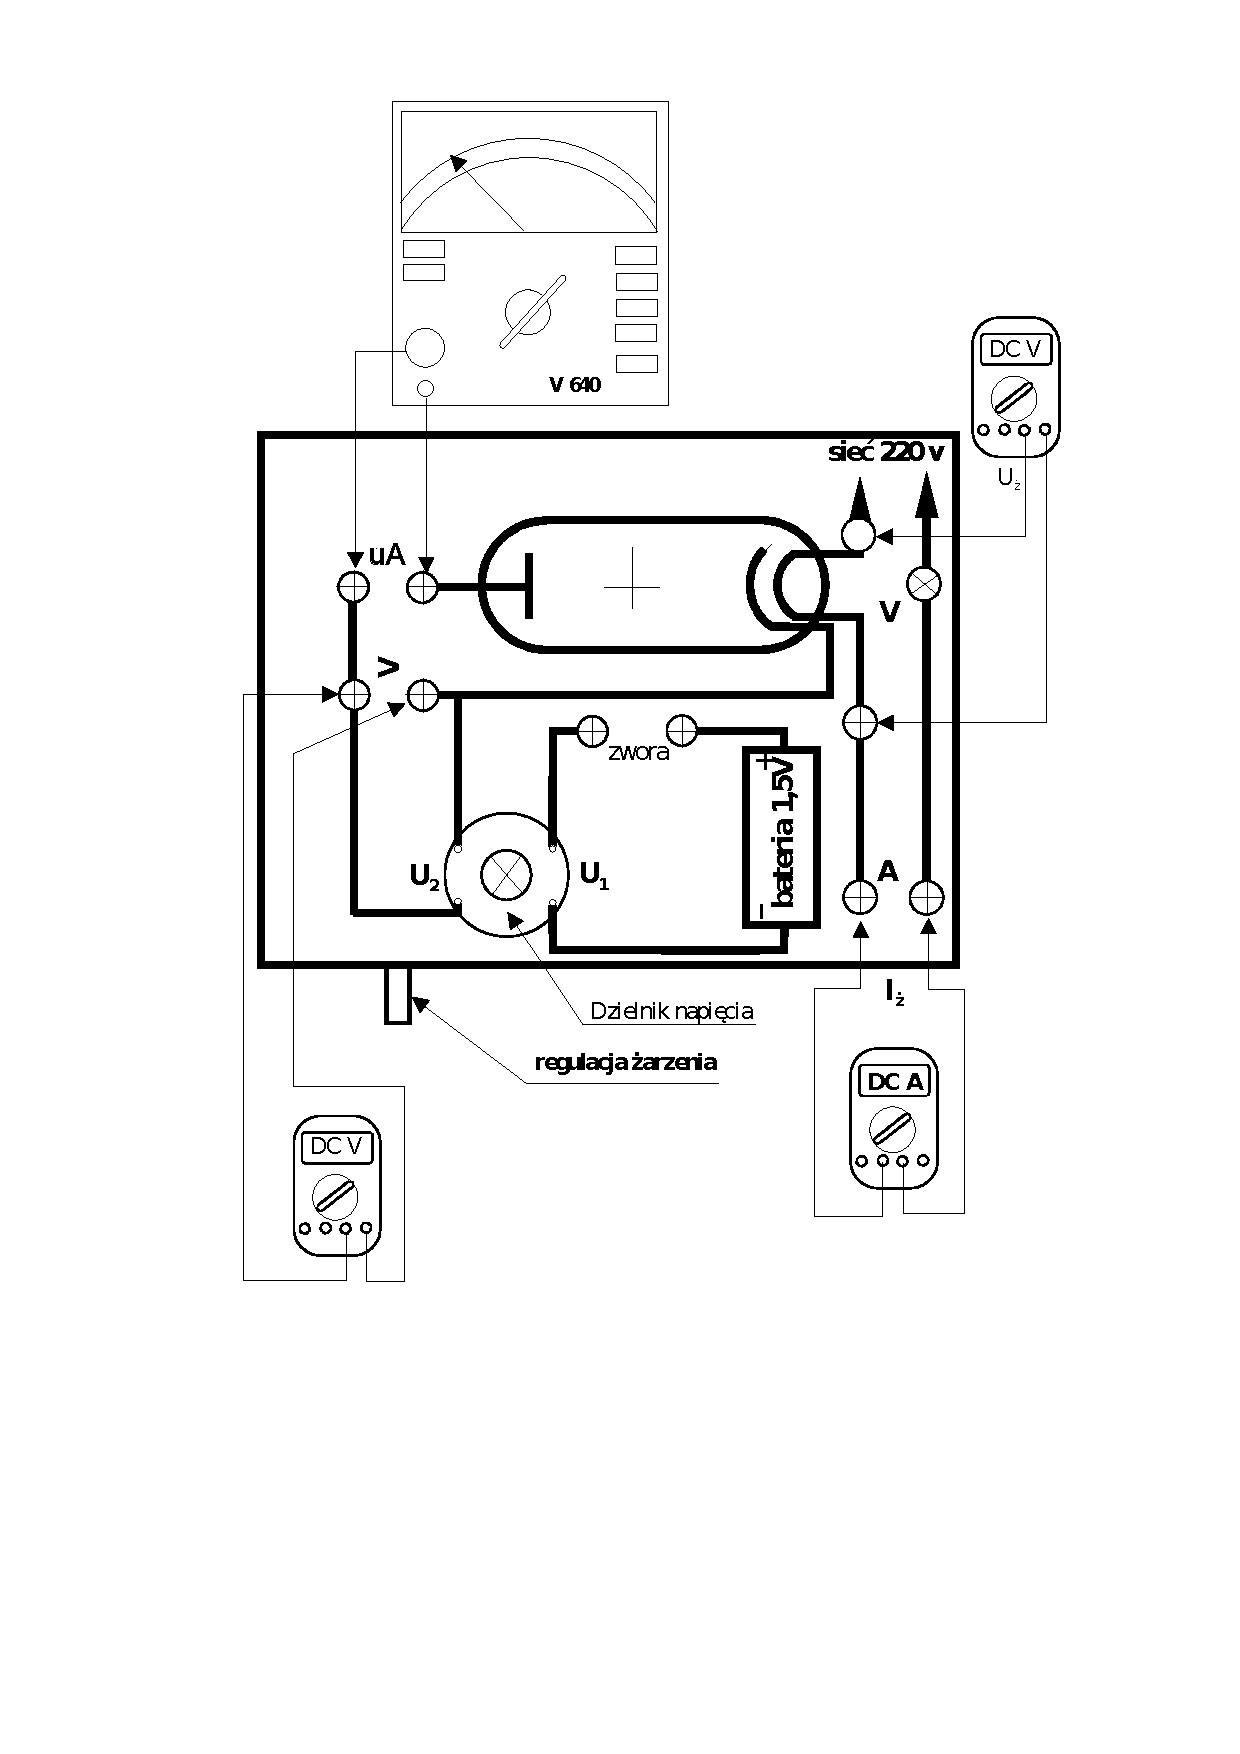
\includegraphics[scale=0.5]{schemat.png}
% \caption{Schemat układu pomiarowego}
% \label{schemat}
% \end{figure}

Układ został przygotowany w taki sposób, aby napięcie przyłożone do lampy elektronowej hamowało
ruch elektronów opuszczających katodę (biegun dodatni baterii połączony został z katodą, a ujemny z anodą).
Budowa układu pozwalała jedynie na regulowanie wartości napięcia \textit{w jedną stronę}.
Z powodu braku możliwości zamiany polaryzacji przykładanego napięcia, nie można było wyznaczyć 
w ćwiczeniu wartości napięcia kontaktowego między okładkami.

Korzystaliśmy z przybliżenia, że elektrony wewnątrz lampy można opisać jako gaz elektronów, oraz dalej, 
z powodu znajdowania się ich w próżni nie występują oddziaływania między nimi -- jako gaz doskonały.
Były to podstawy do założenia, że prędkości elektronów przemieszczających się w kierunku anody 
mają rozkład Maxwella.

Wzór, który uwzględnia ten rozkład i posłużył w ćwiczeniu za podstawę opracowywania wyników pomiarów,
opisuje zależność między natężeniem prądu anodowego a napięciem przyłożonym do lampy.

\begin{align}
	I_a(U_a; T) = I_{a_0} \exp{\left(-\frac{e U_a}{k T}\right)}
\label{eq1}
\end{align}

gdzie $I_a$ to natężenie prądu anodowego, $U_a$ to zmienna niezależna będąca napięciem przyłożonym do lampy,
$T$ to parametr równania, będący temperaturą katody, zaś pozostałe czynniki to następujące stałe:
\begin{itemize}
\item $I_a$ -- prąd \textit{początkowy}
\item $e$ -- ładunek elementrarny z minusem
\item $k$ -- stała Boltzmanna
\end{itemize}

Analizując równanie, mozna stwierdzić, że $I_{a_0}$ to \textit{zerowe} natężenie prądu anodowego przy
braku przyłożonego dodatkowego napięcia ($U_a = 0 \text{V}$). Ponieważ napięcie $U_a$ jest hamujące,
dlatego przyjmuje w naszych rozważaniach wyłącznie wartości ujemne, stąd (pamiętając o ujemnej wartości
ładunku $e$) argument funkcji wykładniczej ma wartość ujemną. Zatem mierzona wartość $I_a$ powinna 
znajdować się w przedziale $(0; I_{a_0}]$ i maleć wraz ze zwiększaniem wartości bezwzględnej
napięcia hamującego. Dodatkowo, wraz ze zwiększaniem temperatury $T$ wykres funkcji wykładniczej
\textit{oddala} się w przedziale $(-\infty; 0)$ od osi $OX$, co wpływa na zwiększenie wartości funkcji
$I_a$ dla ustalonego $x$.

Do dalszego opracowywania wyników wyprowadzono drugi wzór ze wzoru \ref{eq1}, logarytmując równanie
stronami:

\begin{align}
	\ln{\frac{I_a}{I_{a_0}}} = -\frac{e U_a}{k T}
\label{eq2}
\end{align}

Poszukiwana była zależność liniowa, gdzie:
\begin{itemize}
\item $X = U_a$ -- zmienna niezależna
\item $Y = \ln \frac{I_a}{I_{a_0}}$ -- zmienna zależna
\item $a = -\frac{e}{kT}$ -- współczynnik kierunkowy
\end{itemize}





\section{Pomiary i opracowanie wyników}
W naszym doświadczeniu dostaliśmy gotową diodę próżniową oraz mierniki natężenia oraz napięcia, na początku ćwiczenia zmonotowaliśmy obwód w sposób widoczny na rysunku \ref{schemat}. Ustawiliśmy prąd żarzenia na $0.375 A$ przy pierwszym pomiarze oraz $0.385 A$ przy drugim. 
\\ \textbf{Rozkład Maxwella} określa on rozkład prędkości cząstek gazu doskonałego. Określa on liczbę cząstek które w jednostce obiętości mają prędkości z przedziału $<v, v + dv>$. W naszym doświadczeniu wyemitowane elektrony możemy traktować właśnie jako cząstki gazu doskonałego, ponieważ są one emitowane z gęstością o 10-15 rzędów mniejszą niż w metalu, dzięki temu nie oddziaływują ze sobą. 



\begin{table}[h!]
\centering
 \begin{tabular}{ | l | l | l | l | l | l | l | l | }
 \hline
 L.p & $I\_a$ [µA] & $\Delta$ $I\_a$ [mA] & U[V] & $\Delta$ v [mV] & ln $l\_a/l\_a\_0$ & $\Delta$ ln & sqrt \\ \hline
 1 & 0.25 & 0.0168325082306035 & 0 & 0.000577350269189626 & 0 & 0.0952190457139047 & 0 \\ \hline
 2 & 0.2 & 0.0168325082306035 & -0.016 & 0.000605063082110728 & -0.22314355131421 & 0.107780641428165 & 0.126491106406735 \\ \hline
 3 & 0.15 & 0.0168325082306035 & -0.038 & 0.000643168199877243 & -0.510825623765991 & 0.130866061016315 & 0.194935886896179 \\ \hline
 4 & 0.15 & 0.00168325082306035 & -0.041 & 0.00064836435229995 & -0.510825623765991 & 0.0682587669040341 & 0.202484567313166 \\ \hline
 5 & 0.14 & 0.00168325082306035 & -0.047 & 0.000658756657145363 & -0.579818495252942 & 0.0683951106181033 & 0.216794833886788 \\ \hline
 6 & 0.125 & 0.00168325082306035 & -0.055 & 0.000672613063605914 & -0.693147180559945 & 0.0686634303444466 & 0.234520787991171 \\ \hline
 7 & 0.12 & 0.00168325082306035 & -0.058 & 0.000677809216028621 & -0.7339691750802 & 0.0687756686088372 & 0.240831891575846 \\ \hline
 8 & 0.105 & 0.00168325082306035 & -0.069 & 0.000696861774911878 & -0.867500567704723 & 0.0692121739211856 & 0.262678510731274 \\ \hline
 9 & 0.085 & 0.00168325082306035 & -0.085 & 0.00072457458783298 & -1.07880966137193 & 0.0701818366536416 & 0.291547594742265 \\ \hline
 10 & 0.07 & 0.00168325082306035 & -0.1 & 0.000750555349946513 & -1.27296567581289 & 0.0714952070131302 & 0.316227766016838 \\ \hline
 11 & 0.06 & 0.00168325082306035 & -0.112 & 0.00077133995963734 & -1.42711635564015 & 0.0729408689992817 & 0.33466401061363 \\ \hline
 12 & 0.05 & 0.00168325082306035 & -0.125 & 0.000793856620135735 & -1.6094379124341 & 0.0752772652709081 & 0.353553390593274 \\ \hline
 13 & 0.04 & 0.00168325082306035 & -0.141 & 0.000821569433056838 & -1.83258146374831 & 0.0793987825263503 & 0.375499667110372 \\ \hline
 \end{tabular}
\caption{Wyniki wielokrotnych pomiarów i niepwności dla pomiaru drugiego}
\end{table}
% TODO zbyt małe niepewności względem kropek dlatego ich nie widać



\begin{figure}
\centering
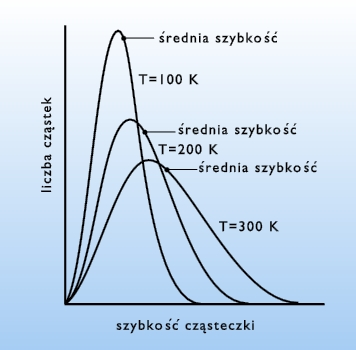
\includegraphics[scale=0.5]{rozlad_maxwella.jpg}
\caption{Rozkład Maxwella \url{zasoby1.open.agh.edu.pl/dydaktyka/chemia/a_e_chemia/2_stany_skupienia/img5/02_02_46.jpg}}
\end{figure}

\subsection{Pierwszy pomiar}
Wyniki pomiarów wykonanych i niepewności dla pierwszego prądu żarzenia są zawarte w tabeli \ref{T1_pomiar}. Niepewność pomiarowa natężenia prądu wyraża się wzorem: 
\begin{align*}
u_{I_{a}} = \sqrt{(\frac{\Delta I}{\sqrt{3}})^2 + (\frac{\Delta I_{E}}{\sqrt{3}})^2}
\end{align*}
gdzie:\\
$u_{I_{a}}$ - niepewność pomiaru wartości natężenia \\
$\Delta I$ - niepewność amperomierza \\
$\Delta I_{E}$ - niepewność eksperymentatora\\

W naszym przypadku amperomierz był wychyłowy i posiadał pierwszą klasę czyli by wyznaczyć $\Delta I$ posłużyliśmy się wzorem:
\begin{align*}
\Delta I = klasa urządzenia * \frac{zakres}{100}
\end{align*}
podanym na wykładzie wstępnym.
Przyjeliśmy że niepewność eksperymentatora jest równa $\frac{1}{2}$ najmniejszej podziałki.\\

Wyniki znajdujące się w kolumnie $u_{U}$ są niepewnościami pomiarowymi napięcia prądu. Wartość niepewności zależy zarówno od jakości urządzenia pomiarowego jak i samego odczytu, w naszym przypadku wyraża się wzorem:
\begin{align*}
u_{U} = \frac{0,3 \% \cdot rdg + 1 \cdot dgt}{\sqrt{3}}
\end{align*}
gdzie: \\
$rdg$ - zmierzona wartość \\
$dgt$ - dokładność pomiaru \\

Wyniki dla niepewności wyznaczenia logarytmu stosunku prądu zmierzonego do prądu początkowego obliczyliśmy z następujacego wzoru:
\begin{align*}
u_{ln} = \sqrt{(\frac{1}{I_{a}})^2 \cdot U_{I_{a}}^2 + (- \frac{1}{I_{a0}})^2 \cdot U_{I_{a0}}^2 }
\end{align*}
gdzie:\\
$u_{ln}$ - niepewność logarytmu stosunku wartości natężenia zmierzonego do prądu początkowego \\
$I_{a}$ - wartość zmierzonego prądu\\
$I_{a0}$ - wartość prądu początkowego\\
$u_{I_{a}}$ - niepewność pomiaru wartości natężenia \\
$u_{I_{a0}}$ - niepewność pomiaru wartości natężenia początkowego \\

W większości punktów na wykresie nie jest widoczna niepewność, ponieważ są one mniejsze od punktów którymi są zaznaczone pomiary.

\begin{table}[h!]
\centering
 \begin{tabular}{ | l | l | l | l | l | l | l | l | }
 \hline
 L.p & $I\_a$ [µA] & $\Delta$ $I\_a$ [mA] & U[V] & $\Delta$ v [mV] & ln $I_{a}$/$I\_a\_0$ & $\Delta$ ln & sqrt \\ \hline
1 & 0.135 & 0.0017 & 0.000 & 0.000577350269189626 & 0 & 0.0176331566136861 & 0 \\ \hline
2 & 0.110 & 0.0017 & -0.012 & 0.000598134878880452 & -0.204794412646013 & 0.0197388927170629 & 0.109544511501033 \\ \hline
3 & 0.105 & 0.0017 & -0.018 & 0.000608527183725866 & -0.251314428280906 & 0.0203090076479504 & 0.134164078649987 \\ \hline
4 & 0.100 & 0.0017 & -0.021 & 0.000613723336148572 & -0.300104592450338 & 0.0209474924373951 & 0.144913767461894 \\ \hline
5 & 0.090 & 0.0017 & -0.030 & 0.000629311793416692 & -0.405465108108164 & 0.0224779524148558 & 0.173205080756888 \\ \hline
6 & 0.080 & 0.0017 & -0.038 & 0.000643168199877243 & -0.523248143764548 & 0.0244575640531662 & 0.194935886896179 \\ \hline
7 & 0.070 & 0.0017 & -0.045 & 0.000655292555530225 & -0.65677953638907 & 0.0270868122635056 & 0.212132034355964 \\ \hline
8 & 0.065 & 0.0017 & -0.055 & 0.000672613063605914 & -0.730887508542792 & 0.0287415299857819 & 0.234520787991171 \\ \hline
9 & 0.055 & 0.0017 & -0.065 & 0.000689933571681603 & -0.897941593205958 & 0.0330469851051302 & 0.254950975679639 \\ \hline
10 & 0.050 & 0.0017 & -0.075 & 0.000707254079757292 & -0.993251773010283 & 0.0358998250610602 & 0.273861278752583 \\ \hline
11 & 0.040 & 0.0017 & -0.089 & 0.000731502791063256 & -1.21639532432449 & 0.0438896051407931 & 0.298328677803526 \\ \hline
12 & 0.035 & 0.0017 & -0.097 & 0.000745359197523807 & -1.34992671694902 & 0.0496828871559356 & 0.311448230047949 \\ \hline
13 & 0.030 & 0.0017 & -0.107 & 0.000762679705599496 & -1.50407739677627 & 0.0574770585036287 & 0.327108544675923 \\ \hline
 \end{tabular}
\caption{Wyniki wielokrotnych pomiarów i niepwności dla pomiaru pierwszego}
\label{T1_pomiar}
\end{table}

\begin{figure}
	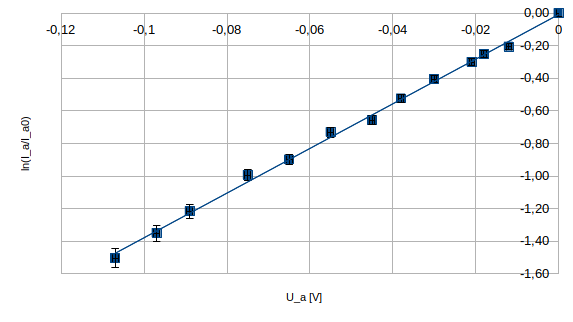
\includegraphics[scale=1]{T1_ln_U}
	\centering
	\caption{Wykres zależności logarytmu stosunku zmierzonego natężenia do natężenia początkowego od napięcia}
\end{figure}

Używając metody najmniejszych kwadratów policzyliśmy temeperaturę katody wysyłającej elektrony. Współczynnik kierunkowy prostej wynosi:
\begin{align*}
a \approx 13.81 (0.11)
\end{align*}

Z tego otrzymujemy temperaturę katody oraz błąd:
\begin{align*}
T = \frac{e}{k \cdot a} \approx 840.36 K
\end{align*}

\begin{align*}
u_{T} = \sqrt{(\frac{e}{k \cdot a^2}) \cdot u_{a}^2} \approx 6.57 K
\end{align*}


\begin{figure}
	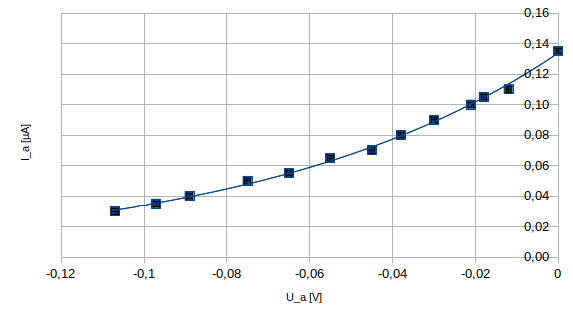
\includegraphics[scale=1]{T1_Ia_U}
	\centering
	\caption{Wykres zależności natężenia od napięcia}
\end{figure}

\begin{figure}
	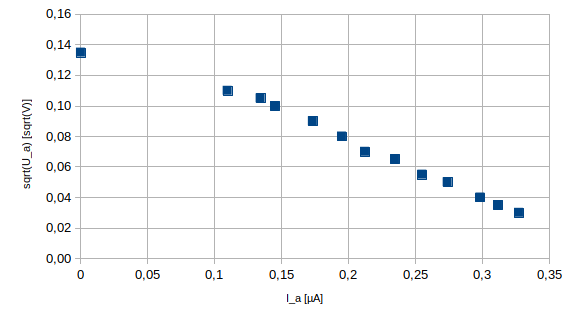
\includegraphics[scale=1]{T1_Ia_sqrtU}
	\centering
	\caption{Wykres zależności natężenia od pierwiastka napięcia}
\end{figure}


\subsection{Drugi pomiar}
W drugim pomierze w przeciwieństwie do pierwszego zmienialiśmy zakres pomiarów na amperomierzu (z tego wynikają większe niepewności pomiarowe dla 3 pierwszych pomiarów). Analogicznie do poprzedniego pomiaru wyznaczyliśmy tempraturę metodą najmniejszych kwadratów. Współczynnik kierunkowy prostej wynosi:
\begin{align*}
a \approx 12.80 (0.06)
\end{align*}

Z tego otrzymujemy temperaturę katody oraz błąd:
\begin{align*}
T \approx 906.31 K
\end{align*}

\begin{align*}
u_{T} = 3.96 K
\end{align*}



\begin{figure}
	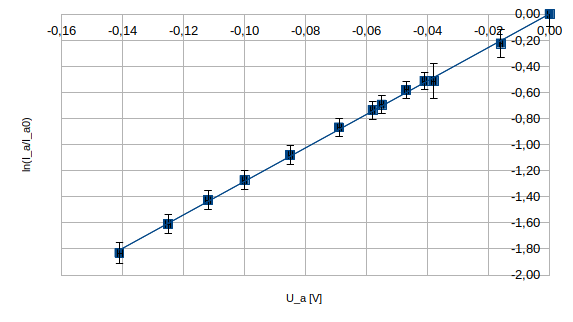
\includegraphics[scale=1]{T2_ln_U}
	\centering
	\caption{Wykres zależności logarytmu stosunku zmierzonego natężenia do natężenia początkowego od napięcia}
\end{figure}

\begin{figure}
	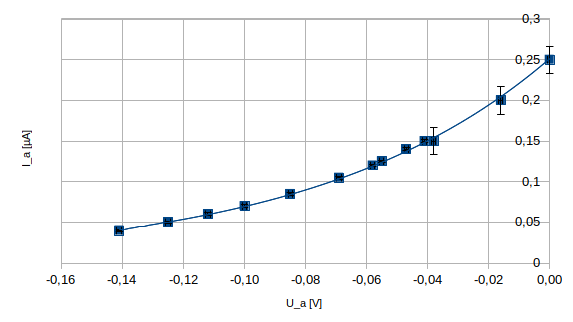
\includegraphics[scale=1]{T2_Ia_U}
	\centering
	\caption{Wykres zależności natężenia od napięcia}
\end{figure}

\begin{figure}
	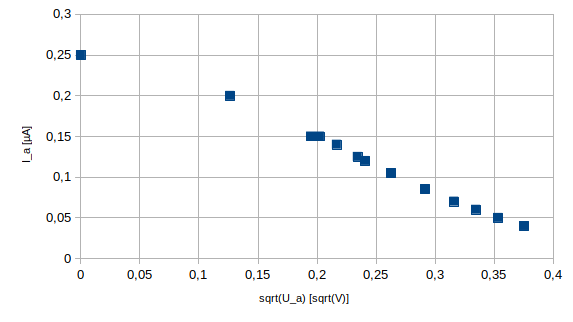
\includegraphics[scale=1]{T2_Ia_sqrtU}
	\centering
	\caption{Wykres zależności natężenia od pierwiastka napięcia}
\end{figure}

\end{document}
